%!TEX root = ../thesis.tex
本章では,開発したロボットアームがオフィス環境で想定される作業に対して,メカニズム的に問題がないかを検証する.また,安全対策の検討を行う.
\section{検証方法}
第\ref{chap:second}章で行った作業調査の結果,本研究で開発したロボットアームの検証として,「机の片づけ作業」が適していると判断した.これを踏まえ,本検証では,机の片づけ作業を想定して検証を行った.
検証環境を図\ref{fig:area}に示す.50×100の範囲にランダムに紙コップを配置した.図\ref{fig:area}の黄色テープの位置にロボットアームの肩ヨー軸を置き,人間がロボットアームを支えて手先を動かす.検証の様子を図\ref{fig:sousa}に示す.
この検証を通し,ロボットアームの手先が干渉なく紙コップにアプローチできるかを確認する.

\begin{figure}
  \centering
  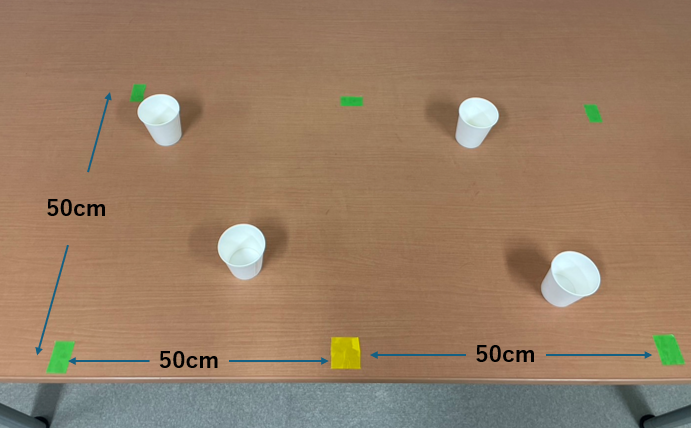
\includegraphics[width=10cm]{images/kensyo/area.png}
  \caption{Test environment: Randomly place paper cups in a 50 x 100 area}
  \label{fig:area}
\end{figure}
\begin{figure}
  \centering
  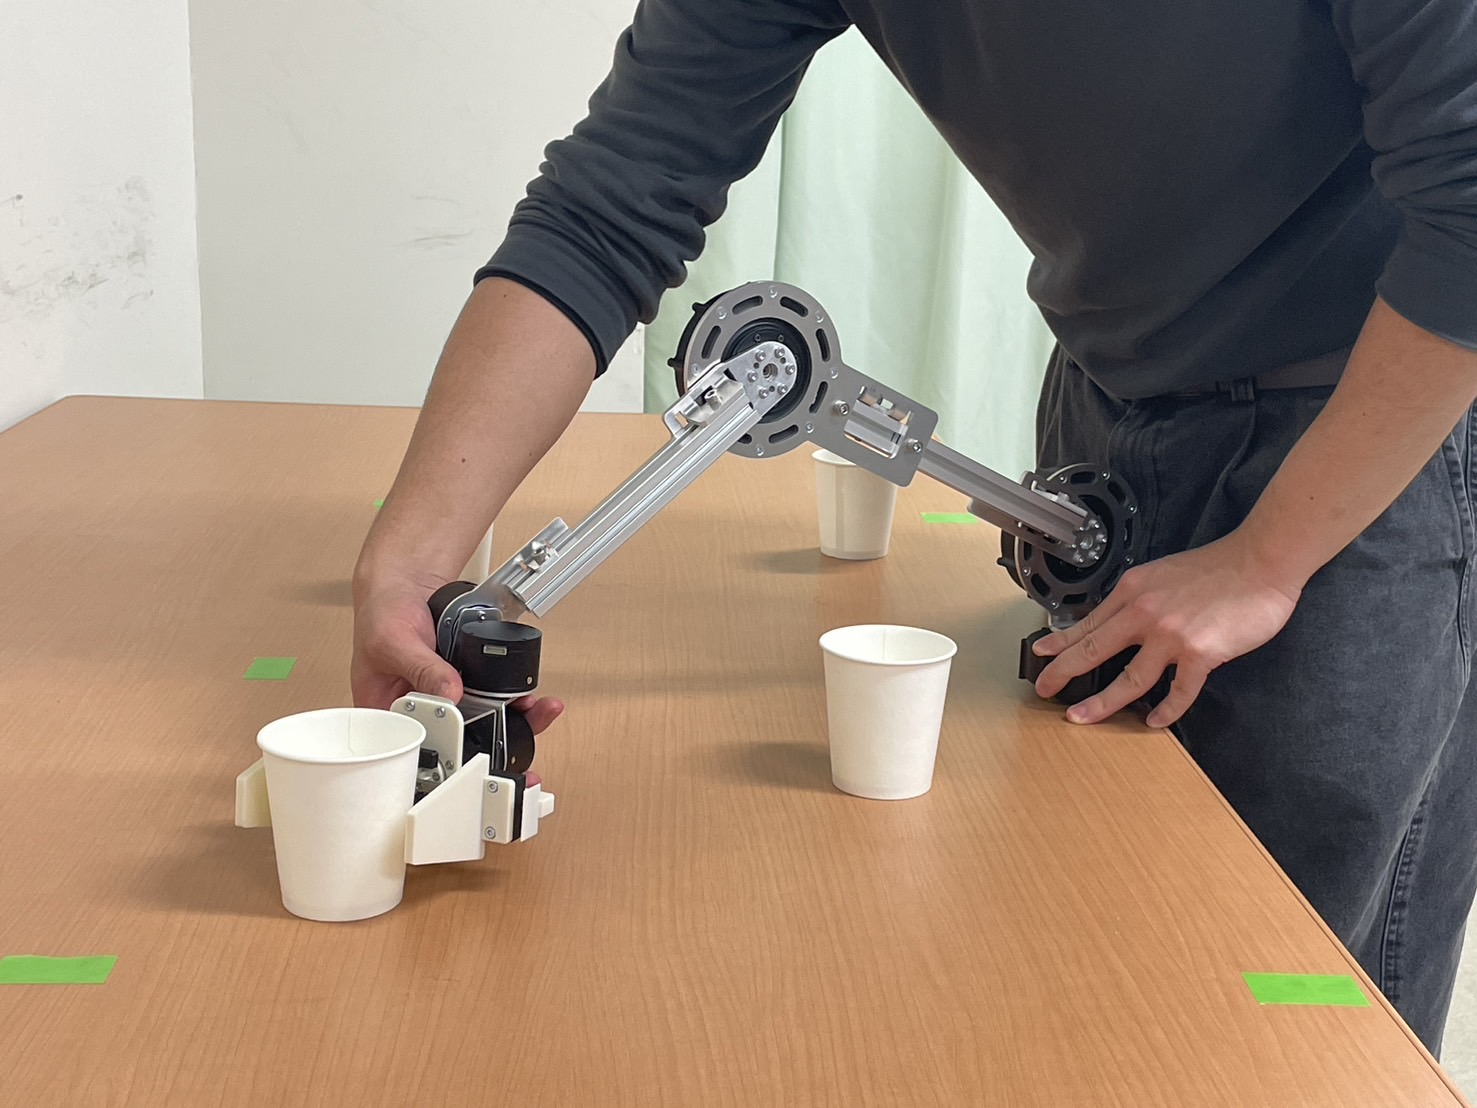
\includegraphics[width=10cm]{images/kensyo/sousa.jpg}
  \caption{How a robot arm is supported and moved by a person}
  \label{fig:sousa}
\end{figure}
\clearpage
\section{検証結果}
本検証は10回の試行を実施し,すべての試行で問題なく動作することを確認した.構造設計時に確認された作業領域では,ロボットアームの根元付近にある物体へのアプローチが困難であるという問題が発生していた.この原因は,「物体を正面から掴む」という条件を設けていたためであった.一方,本検証では,ハンドの角度を固定することが困難であったため,この条件を撤廃して実施した.その結果,図\ref{fig:tikai}に示すように,ロボットアームに近い位置にある物体にも干渉なくアプローチ可能であることが確認された.

しかし,この結果は,作業領域の拡大という課題が解消されたことを意味するものではない.今回の検証では,紙コップのような筒状の物体を対象としたため,どの方向から掴んでも形状が変わらず,干渉の問題が発生しなかった.しかし,箱型の物体や取っ手のある物体など,掴む方向に制限がある場合には,ロボットアームが干渉し動作が困難になることが予想される.

したがって,作業領域の拡大という課題は依然として残されており,今後の検討が必要である.
\begin{figure}
  \centering
  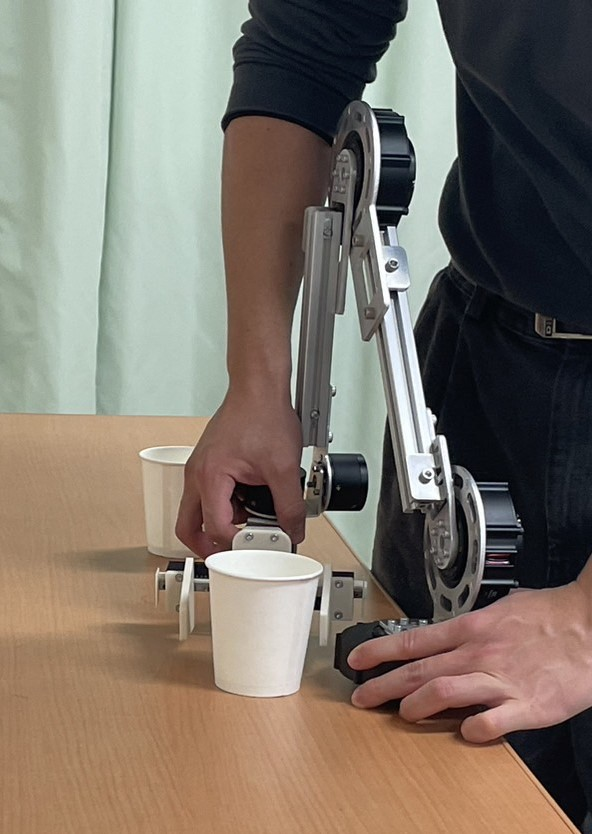
\includegraphics[width=8cm]{images/kensyo/tikai.jpg}
  \caption{Approaching a paper cup near the robot arm}
  \label{fig:tikai}
\end{figure}
\newpage

\section{安全対策の検討}
本節では,ロボットアームが通電した際に必要な安全対策について検討する.本ロボットアームはQDDモータを採用しており,高トルクおよび高スピードという特性を有するが,これらの特性は暴走時に大きなリスクを伴う.したがって,以下では,通電状態での安全な運用を実現するために必要な対策を検討する.

まず,ロボットアームの可動範囲内への進入を防止することが挙げられる.本ロボットアームの重量は約2.2kgであり,高スピードで動作中に接触が発生した場合,大事故につながる可能性がある.適切で完全な制御が確立するまでは,可動範囲内に人が入らないようにすることが必要である.

次に,暴走時に遠隔で動作停止が可能なシステムの構築が重要である.暴走が発生した場合,人がロボットアームに近づくことは困難であるため,離れた位置からロボットアームを停止できる仕組みが求められる.これにより,暴走による被害を最小限に抑えることが可能となる.

以上のように,QDDモータは適切な制御を行うことで安全性を高める可能性を持つ一方で,不適切な運用が人に危害を及ぼすリスクを伴う.そのため,ロボットアームの動作時には,最低限,以下の2点を満たす安全対策が必要である

\begin{enumerate}
  \item 可動範囲内への進入を防止する仕組み
  \item 遠隔で動作停止が可能なシステムの導入
\end{enumerate}

これらの対策を講じることが,QDDモータを搭載したロボットアームの安全な運用に不可欠であると考える.